\begin{frame}{Procedures}
    Procedures, Subroutines, Functions, Methods, etc. let us abstract away the algo implementation.\\
    Only need to implement code once.
\end{frame}

\subsection{Procedure Declarations}
\begin{frame}{Procedure Declarations}
    Our procedures have been inspired by PASCAL.\\
    Our procedure declerations have;
    \begin{itemize}[<+->]
        \item List of params
        \item local vars
        \item code
    \end{itemize}
\end{frame}

\begin{frame}{Procedure Declarations}
    See script 5.1
\end{frame}

\subsubsection*{Parameters \& Local Variables}
\begin{frame}{Parameters \& Local Variables}
    \begin{itemize}
        \item Local variables are vars that are declared and used only within the procedure.
        \item Parameters are local vars that are instantiated with the value/reference of arg.
    \end{itemize}
    Parameters also specify \textit{how} the procedure communicats with the outside world.
\end{frame}

\subsubsection*{Performing a Procedure}
\begin{frame}{Performing a Procedure}
    Performing a procedure is done in the following steps
    \begin{enumerate}[<+->]
        \item The first is that we need to somehow remember the current environment or delete all the local variables when we're done. The best way is to get the current stack frame.
        \item We then add all the local variables.
        \item We then execute the procedure statements.
        \item We then reset the environment back to how it looked before using the saved stack frame from (1). This ensures that all local variables
        that shouldn't exist outside the procedure are removed. 
    \end{enumerate}
\end{frame}

\subsubsection*{Executing a procedure call}
\begin{frame}{Executing a Procedure Call}
    We have now established how to perform a procedure.\\
    We need to set up the environment for it first.
\end{frame}
\subsection{Argument pasing}
\begin{frame}{Argument Passing}
    \begin{itemize}[<+->]
        \item Copy Semantics
        \item Reference Semantics
    \end{itemize}
\end{frame}

\subsection*{Q\&A}
\begin{frame}{Questions?}
    \begin{figure}
        \centering
        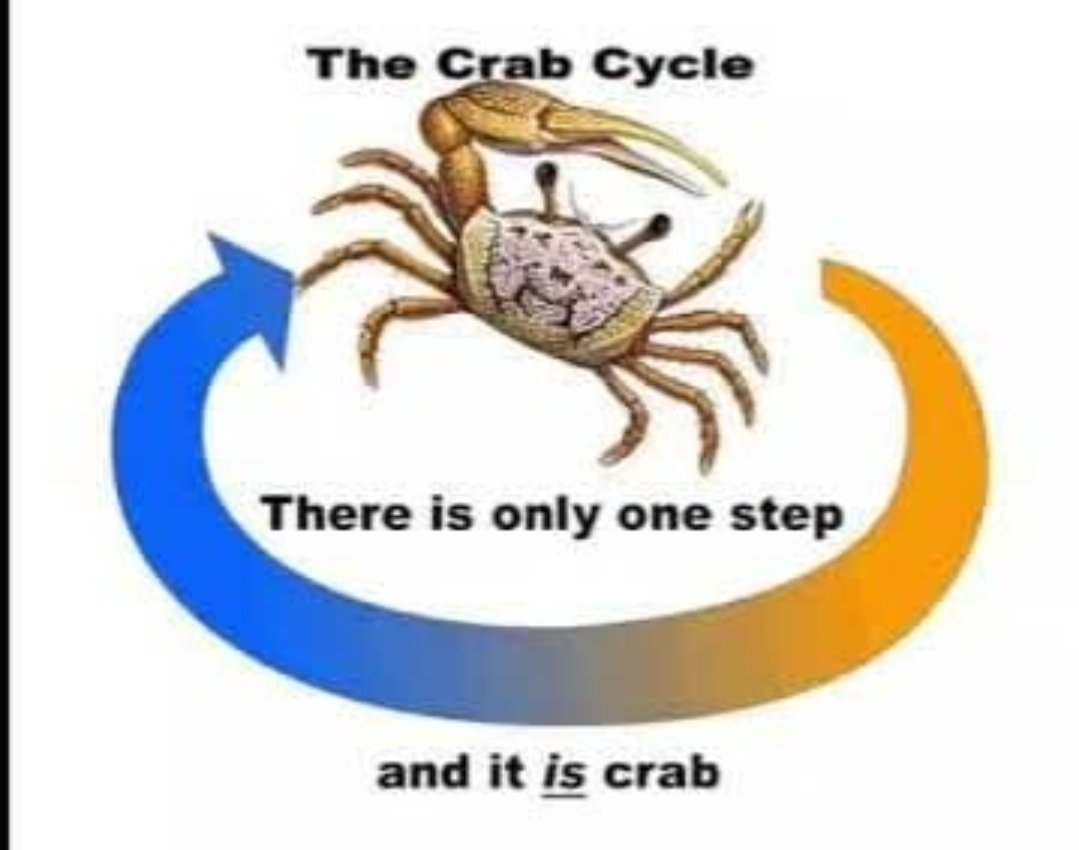
\includegraphics[height = 4.9cm]{intermission/chap05.jpg}
    \end{figure}
\end{frame}